\documentclass[10pt,a4paper]{article}

\usepackage[a4paper, top=22mm, bottom=22mm, left=20mm, right=20mm]{geometry}
\usepackage{tikz}
\usetikzlibrary{shapes.geometric,arrows.meta,positioning,fit,backgrounds,calc,automata}
\usepackage{booktabs,array,tabularx,multirow,xcolor,colortbl,enumitem}
\usepackage{titlesec,fancyhdr,amsmath,parskip,hyperref,caption,pifont,makecell}

%% ── palette: two accent colours, rest greyscale ─────────────────────────────
\definecolor{acc1}{RGB}{41,98,148}      % steel blue  — section rules, emph borders
\definecolor{acc2}{RGB}{230,115,0}      % amber       — CDC bar, DFI bar, warnings
\definecolor{acc3}{RGB}{34,120,100}     % teal        — group box fills
\definecolor{ruleclr}{RGB}{185,185,185}
\definecolor{hdrclr}{RGB}{20,20,20}
\definecolor{thbg}{RGB}{225,232,240}    % table header: very pale blue
\definecolor{altbg}{RGB}{249,250,251}
\definecolor{boxbdr}{RGB}{155,155,155}
\definecolor{boxfill}{RGB}{245,247,250}
\definecolor{acc1lt}{RGB}{225,235,245}  % pale blue fill
\definecolor{acc2lt}{RGB}{255,243,225}  % pale amber fill
\definecolor{acc3lt}{RGB}{220,240,235}  % pale teal fill
\definecolor{notetext}{RGB}{90,90,90}
\definecolor{imgbg}{RGB}{247,248,249}

\hypersetup{colorlinks=false,hidelinks}

%% ── page style ───────────────────────────────────────────────────────────────
\pagestyle{fancy}\fancyhf{}
\fancyhead[L]{\small\textbf{\color{acc1}DDR Memory Controller}\enspace
              {\normalfont\color{notetext}MC Core Design Specification}}
\fancyhead[R]{\small\color{notetext}JESD79-5 / DFI\,5.2 / AXI4\quad\thepage}
\renewcommand{\headrulewidth}{0.5pt}
\renewcommand{\headrule}{\color{acc1}\hrule height 0.5pt}

%% ── section style ────────────────────────────────────────────────────────────
\titleformat{\section}{\normalsize\bfseries\color{acc1}}{\thesection}{0.6em}{}
  [\vspace{1pt}\color{acc1!40}\hrule height 0.5pt\vspace{2pt}]
\titlespacing{\section}{0pt}{14pt}{4pt}
\titleformat{\subsection}{\small\bfseries\color{hdrclr}}{\thesubsection}{0.5em}{}
\titlespacing{\subsection}{0pt}{8pt}{2pt}
\titleformat{\subsubsection}{\small\itshape\color{notetext}}{\thesubsubsection}{0.5em}{}
\titlespacing{\subsubsection}{0pt}{5pt}{1pt}

%% ── lists ────────────────────────────────────────────────────────────────────
\setlist[itemize]{itemsep=1pt,topsep=2pt,parsep=0pt,label={\color{acc1}--}}
\setlist[itemize,2]{label={\color{notetext}$\circ$},leftmargin=1.4em}
\setlist[enumerate]{itemsep=1pt,topsep=2pt,parsep=0pt}

%% ── table macros ─────────────────────────────────────────────────────────────
\newcommand{\Th}[1]{\cellcolor{thbg}\textbf{\small\color{acc1}#1}}
\newcommand{\RA}{\rowcolor{white}}
\newcommand{\RB}{\rowcolor{altbg}}
\arrayrulecolor{ruleclr}
\setlength{\tabcolsep}{5pt}
\renewcommand{\arraystretch}{1.22}

%% ── TikZ ─────────────────────────────────────────────────────────────────────
\tikzset{
  %% standard block
  mblk/.style={rectangle,rounded corners=2pt,draw=boxbdr,fill=boxfill,
    minimum width=2.0cm,minimum height=0.62cm,
    font=\scriptsize,align=center,text=hdrclr,inner sep=4pt},
  %% accent blue block (MC core internals)
  ablk/.style={rectangle,rounded corners=2pt,draw=acc1!60,fill=acc1lt,
    minimum width=2.0cm,minimum height=0.62cm,
    font=\scriptsize,align=center,text=acc1,inner sep=4pt},
  %% amber block (CDC / DFI interface bars)
  amblk/.style={rectangle,rounded corners=2pt,draw=acc2!70,fill=acc2lt,
    minimum width=5.0cm,minimum height=0.62cm,
    font=\scriptsize\bfseries,align=center,text=acc2,inner sep=4pt},
  %% teal block (CIF / PHY)
  tblk/.style={rectangle,rounded corners=2pt,draw=acc3!60,fill=acc3lt,
    minimum width=5.0cm,minimum height=0.62cm,
    font=\scriptsize\bfseries,align=center,text=acc3,inner sep=4pt},
  %% group bounding box
  grpbox/.style={rectangle,rounded corners=3pt,draw=#1!50,
    fill=#1!4,dashed,inner sep=8pt},
  %% FSM state circle
  st/.style={circle,draw=acc1!60,fill=acc1lt,minimum size=1.0cm,
    font=\tiny\bfseries,align=center,text=acc1},
  %% arrows
  arr/.style={-Stealth,thin,color=hdrclr},
  darr/.style={-Stealth,thin,dashed,color=notetext},
  aarr/.style={-Stealth,thin,color=acc2},
  lbl/.style={font=\tiny,color=notetext,align=center},
  %% image placeholder box
  imgbox/.style={rectangle,draw=ruleclr,fill=imgbg,rounded corners=3pt,
    minimum height=5.0cm,align=center,text=notetext,
    font=\small\itshape,inner sep=8pt},
}

\captionsetup{font={small,color=notetext},labelfont={bf,color=acc1},
  labelsep=period,skip=4pt}
\setlength{\parindent}{0pt}
\setlength{\parskip}{3.5pt}

%%%%%%%%%%%%%%%%%%%%%%%%%%%%%%%%%%%%%%%%%%%%%%%%%%%%%%%%%%%%%%%%%%%%%%%%%%%%
\begin{document}
%%%%%%%%%%%%%%%%%%%%%%%%%%%%%%%%%%%%%%%%%%%%%%%%%%%%%%%%%%%%%%%%%%%%%%%%%%%%

%% ── title ────────────────────────────────────────────────────────────────────
\begin{flushleft}
  {\large\bfseries\color{acc1} Reconfigurable DDR5 Memory Controller}\\[2pt]
  {\normalsize\bfseries MC Core\,---\,Design Specification}\\[3pt]
  {\small\color{notetext}Sub-Blocks $\cdot$ FSMs $\cdot$ Timing Constraints $\cdot$
   DFI\,5.2 Interface}
\end{flushleft}
\noindent\color{acc1}\rule{\linewidth}{0.7pt}
\smallskip
\begin{tabular}{@{}ll@{\quad}ll@{\quad}ll@{}}
\small\textbf{Standard} & \small JEDEC JESD79-5, DFI\,5.2, AXI4 &
\small\textbf{Burst}    & \small BL16 (BL/2\,=\,8\,clk) &
\small\textbf{FSMs}     & \small 23 total \\
\small\textbf{Banks}    & \small 16 (2\,BG\,$\times$\,4 banks) &
\small\textbf{Clock}    & \small Dual: AXI\,/\,MC (CDC at one crossing) &
\small\textbf{DFI ratio}& \small 1:1, 1:2, 1:4 \\
\end{tabular}
\vspace{2pt}\noindent\color{ruleclr}\rule{\linewidth}{0.4pt}

%%%%%%%%%%%%%%%%%%%%%%%%%%%%%%%%%%%%%%%%%%%%%%%%%%%%%%%%%%%%%%%%%%%%%%%%%%%%
\section{System Overview}
%%%%%%%%%%%%%%%%%%%%%%%%%%%%%%%%%%%%%%%%%%%%%%%%%%%%%%%%%%%%%%%%%%%%%%%%%%%%

The MC Core sits entirely in the MC clock domain, receiving commands from the Client
Interface (CIF) via a single Async FIFO CDC bar, and emitting DFI\,5.2 commands to the
DDR PHY. Every DRAM timing constraint, scheduling decision, refresh housekeeping, and
power-state transition is the MC Core's responsibility. It has no knowledge of the AXI
protocol --- that is fully resolved by the CIF upstream.

\subsection{Full Microarchitecture Block Diagram}

% ── IMAGE PLACEHOLDER: paste Figure 2 from the reference PDF here ────────────
\begin{figure}[h]
\centering
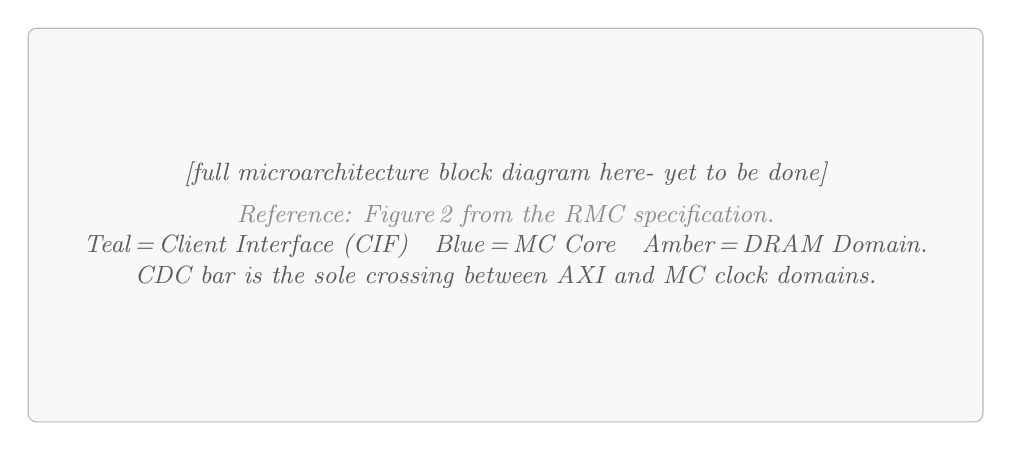
\begin{tikzpicture}
  \node[imgbox,minimum width=\linewidth]
    {[full microarchitecture block diagram here- yet to be done]\\[4pt]
     \small\color{notetext!70}
     Reference: Figure\,2 from the RMC specification.\\
     Teal\,=\,Client Interface (CIF)\quad
     Blue\,=\,MC Core\quad
     Amber\,=\,DRAM Domain.\\
     CDC bar is the sole crossing between AXI and MC clock domains.};
\end{tikzpicture}
\caption{Full microarchitecture block diagram of the RMC.}
\end{figure}

\subsection{Sub-Block Inventory}

\begin{center}
\begin{tabularx}{\linewidth}{@{} l l X @{}}
\toprule
\Th{Sub-Block} & \Th{Domain} & \Th{Function} \\
\midrule
\RA Config Registers   & MC & All timing parameters, page policy, refresh mode, RFM thresholds, DFI offsets. Written via AXI4-Lite CSR path. \\
\RB Init FSM           & MC & Full DDR5 power-up: RESET\_n, NOP burst, DLL reset, ZQcal via MPC, MRW burst, optional training dispatch. Single instance. \\
\RA Bank State Machines& MC & 16 instances. Tracks bank state, owns all per-bank timers. Source of truth for bank availability. \\
\RB Timing Control     & MC & Combinational + registered timer array. Produces \texttt{cmd\_ok[15:0][cmd\_type]} each cycle for the Scheduler. \\
\RA Arbitration Logic  & MC & Picks winner command class each cycle. Priority, age-based anti-starvation, watermark RD/WR mode switching. \\
\RB Command Selector   & MC & Takes winner class, applies timing constraints, enforces page policy, emits \texttt{\{cmd,\,rank,\,BG,\,bank,\,row,\,col\}}. \\
\RA Refresh Scheduler  & MC & Leaky-bucket tREFI tracking. REFab and REFsb. Up to 8$\times$ postponement; \texttt{ref\_urgent} on overflow. \\
\RB ZQcal FSM          & MC & Periodic MPC ZQCAL Start/Latch sequence. \\
\RA RFM FSM            & MC & DDR5 rowhammer mitigation. Per-bank RAA counters; triggers RFM when RAA\,$\leq$\,RAAIMT. \\
\RB Power Mgmt FSM     & MC & CKE-controlled transitions: Active PD, Precharge PD, Self-Refresh, MPSM. \\
\RA Write Data Path    & MC & BL16-aligned write buffer, DM/ECC generator, Write CRC (CRC-8), DFI write timing pipeline. \\
\RB Read Data Path     & MC & Read capture FIFO, Read CRC/ECC checker, read latency counter, ECS FSM. \\
\bottomrule
\end{tabularx}
\end{center}

%%%%%%%%%%%%%%%%%%%%%%%%%%%%%%%%%%%%%%%%%%%%%%%%%%%%%%%%%%%%%%%%%%%%%%%%%%%%
\section{Config Registers}
%%%%%%%%%%%%%%%%%%%%%%%%%%%%%%%%%%%%%%%%%%%%%%%%%%%%%%%%%%%%%%%%%%%%%%%%%%%%

All timing parameters consumed by the MC Core live here. Programmed before
\texttt{INIT\_KICK}; may be updated at runtime only while the controller is idle.
The Scheduler reads timing values combinatorially every cycle.

\begin{center}
\begin{tabularx}{\linewidth}{@{} l l X @{}}
\toprule
\Th{Register} & \Th{Width} & \Th{Description} \\
\midrule
\RA \texttt{CL}              & 7b  & CAS Latency (nCK). Drives RL in RTW formula. \\
\RB \texttt{CWL}             & 7b  & CAS Write Latency $=$ CL$-$2 (fixed in DDR5). \\
\RA \texttt{tRCD}            & 8b  & RAS-to-CAS delay. ACT to first RD/WR on same bank. \\
\RB \texttt{tRP}             & 8b  & Row Precharge Time. PRE to next ACT on same bank. \\
\RA \texttt{tRAS}            & 9b  & Row Active Time minimum. ACT to PRE minimum. \\
\RB \texttt{tRC}             & 9b  & Row Cycle Time $=$ tRAS$+$tRP. ACT-to-ACT same bank. \\
\RA \texttt{tWR}             & 8b  & Write Recovery Time. WR burst end to PRE. \\
\RB \texttt{tRTP}            & 6b  & Read-to-Precharge. RD cmd to PRE on same bank. \\
\RA \texttt{tCCD\_L}         & 5b  & CAS-to-CAS, same BG (nCK). \\
\RB \texttt{tCCD\_S}         & 5b  & CAS-to-CAS, diff BG $=$ BL/2 $=$ 8\,nCK. \\
\RA \texttt{tCCD\_L\_WR}     & 6b  & WR-to-WR same BG. $\max(32\,\text{nCK},\,20\,\text{ns})$. \\
\RB \texttt{tCCD\_L\_WR2}    & 6b  & WR-to-WR same BG, 2nd not RMW. $\max(16\,\text{nCK},\,10\,\text{ns})$. \\
\RA \texttt{tWTR\_L/tWTR\_S} & 6b/5b & Write-to-Read same/diff BG. \\
\RB \texttt{tRRD\_L/tRRD\_S} & 5b/4b & ACT-to-ACT same/diff BG. \\
\RA \texttt{tFAW}            & 6b  & Four-Activate Window (nCK). \\
\RB \texttt{tRFC1}           & 12b & REFab recovery time. 195\,ns for 8\,Gb DDR5. \\
\RA \texttt{tRFCsb}          & 11b & REFsb per-bank recovery time. \\
\RB \texttt{tREFI}           & 14b & Average refresh interval. 3.9\,$\mu$s at $\leq$85\textdegree C. \\
\RA \texttt{tMRD}            & 5b  & MRW-to-MRW minimum. 16\,nCK in DDR5. \\
\RB \texttt{tXP / tXS}       & 5b/12b & PDX-to-command / SRX-to-command. \\
\RA \texttt{tCKSRE/tCKSRX}   & 5b  & Stable clock after/before SR entry/exit. \\
\RB \texttt{tDLLK}           & 11b & DLL lock time. 1024\,nCK. \\
\RA \texttt{RAAIMT/RAAMMT}   & 8b  & RFM RAA Initial/Maximum Management Threshold (from MR58). \\
\RB \texttt{RAADec}          & 4b  & RAA decrement per REF command issued. \\
\RA \texttt{REF\_MODE}       & 2b  & 00=REFab, 01=REFsb, 10=FGR-2$\times$, 11=FGR-4$\times$. \\
\RB \texttt{PAGE\_POLICY}    & 2b  & 00=Open, 01=Closed, 10=Adaptive. \\
\RA \texttt{AGE\_THR1/2}     & 8b  & Intra/cross-class age escalation thresholds. \\
\RB \texttt{WR\_HIGH/LOW\_WM}& 6b  & Write pool watermarks (default 32 / 8). \\
\RA \texttt{PHY\_WRLAT}      & 6b  & \texttt{dfi\_t\_phy\_wrlat}: WL pipeline offset to PHY. \\
\RB \texttt{PHY\_RDLAT}      & 6b  & \texttt{dfi\_t\_rddata\_en}: RL pipeline offset to PHY. \\
\RA \texttt{FREQ\_RATIO}     & 2b  & DFI frequency ratio: 00=1:1, 01=1:2, 10=1:4. \\
\RB \texttt{INIT\_KICK}      & 1b  & Write 1 to trigger Init FSM. \\
\RA \texttt{SOFT\_RESET}     & 1b  & Synchronous soft-reset of all MC Core FSMs. \\
\bottomrule
\end{tabularx}
\end{center}

%%%%%%%%%%%%%%%%%%%%%%%%%%%%%%%%%%%%%%%%%%%%%%%%%%%%%%%%%%%%%%%%%%%%%%%%%%%%
\section{Init FSM}
%%%%%%%%%%%%%%%%%%%%%%%%%%%%%%%%%%%%%%%%%%%%%%%%%%%%%%%%%%%%%%%%%%%%%%%%%%%%

Reference: JESD79-5 \S3.3.1/3.3.2. Single instance. Triggered by \texttt{INIT\_KICK}.
Emits DFI commands directly, bypassing the Cmd Scheduler. Asserts \texttt{init\_done}
on completion.

\subsection{State Diagram}

\begin{figure}[h]
\centering
% Three-row layout, left-to-right then snake down — no overlapping text
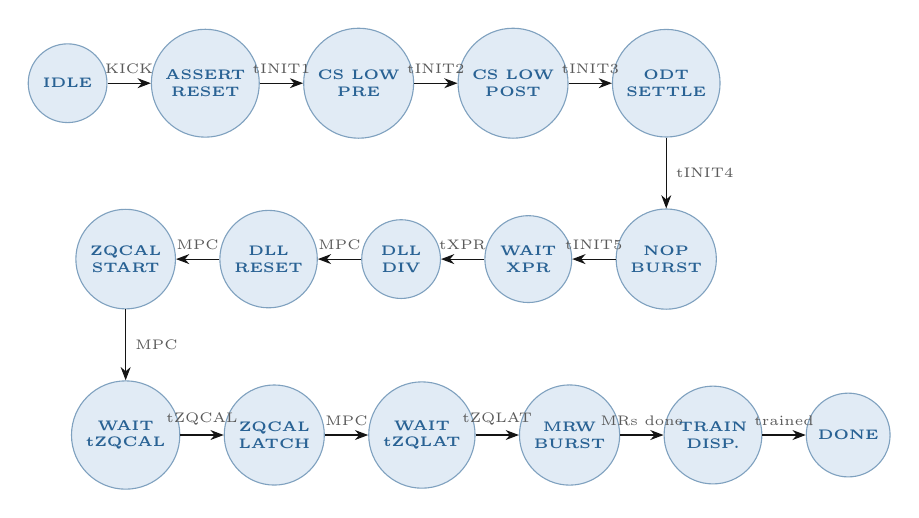
\begin{tikzpicture}[node distance=0.5cm and 0.55cm,
  every node/.style={font=\tiny}]

  %% Row 1 (left to right)
  \node[st] (idle)  {IDLE};
  \node[st,right=0.55cm of idle]  (rst)  {ASSERT\\RESET};
  \node[st,right=0.55cm of rst]   (pre)  {CS LOW\\PRE};
  \node[st,right=0.55cm of pre]   (post) {CS LOW\\POST};
  \node[st,right=0.55cm of post]  (odt)  {ODT\\SETTLE};

  %% Row 2 (right to left)
  \node[st,below=0.9cm of odt]   (nop)  {NOP\\BURST};
  \node[st,left=0.55cm of nop]   (xpr)  {WAIT\\XPR};
  \node[st,left=0.55cm of xpr]   (dlld) {DLL\\DIV};
  \node[st,left=0.55cm of dlld]  (dllr) {DLL\\RESET};
  \node[st,left=0.55cm of dllr]  (zqs)  {ZQCAL\\START};

  %% Row 3 (left to right)
  \node[st,below=0.9cm of zqs]   (wzq)  {WAIT\\tZQCAL};
  \node[st,right=0.55cm of wzq]  (zql)  {ZQCAL\\LATCH};
  \node[st,right=0.55cm of zql]  (wzl)  {WAIT\\tZQLAT};
  \node[st,right=0.55cm of wzl]  (mrw)  {MRW\\BURST};
  \node[st,right=0.55cm of mrw]  (trn)  {TRAIN\\DISP.};
  \node[st,right=0.55cm of trn]  (done) {DONE};

  %% Row 1 arrows
  \draw[arr] (idle)--(rst)   node[above,lbl,midway]{KICK};
  \draw[arr] (rst)--(pre)    node[above,lbl,midway]{tINIT1};
  \draw[arr] (pre)--(post)   node[above,lbl,midway]{tINIT2};
  \draw[arr] (post)--(odt)   node[above,lbl,midway]{tINIT3};

  %% Row 1 -> Row 2 turn
  \draw[arr] (odt.south)--(nop.north) node[right,lbl,midway]{tINIT4};

  %% Row 2 arrows
  \draw[arr] (nop)--(xpr)    node[above,lbl,midway]{tINIT5};
  \draw[arr] (xpr)--(dlld)   node[above,lbl,midway]{tXPR};
  \draw[arr] (dlld)--(dllr)  node[above,lbl,midway]{MPC};
  \draw[arr] (dllr)--(zqs)   node[above,lbl,midway]{MPC};

  %% Row 2 -> Row 3 turn
  \draw[arr] (zqs.south)--(wzq.north) node[right,lbl,midway]{MPC};

  %% Row 3 arrows
  \draw[arr] (wzq)--(zql)    node[above,lbl,midway]{tZQCAL};
  \draw[arr] (zql)--(wzl)    node[above,lbl,midway]{MPC};
  \draw[arr] (wzl)--(mrw)    node[above,lbl,midway]{tZQLAT};
  \draw[arr] (mrw)--(trn)    node[above,lbl,midway]{MRs done};
  \draw[arr] (trn)--(done)   node[above,lbl,midway]{trained};

\end{tikzpicture}
\caption{Init FSM state sequence (JESD79-5 \S3.3.1). Executes once on INIT\_KICK;
         idles until SOFT\_RESET. DFI commands issued directly, bypassing Scheduler.}
\end{figure}

\subsection{State Descriptions}

\begin{center}
\begin{tabularx}{\linewidth}{@{} l X l @{}}
\toprule
\Th{State} & \Th{Action} & \Th{Exit} \\
\midrule
\RA IDLE                & Hold RESET\_n=0, CKE=0, CS\_n=0. & INIT\_KICK=1 \\
\RB ASSERT\_RESET       & RESET\_n LOW. CS\_n LOW. Load tINIT1 (200\,$\mu$s). & tINIT1 expires \\
\RA CS\_LOW\_PRE        & CS\_n LOW. Wait tINIT2 (10\,ns) before releasing RESET\_n. & tINIT2 expires \\
\RB CS\_LOW\_POST       & Deassert RESET\_n. CS\_n LOW. CKE LOW. Count tINIT3 (4\,ms). & tINIT3 expires \\
\RA ODT\_SETTLE         & Raise CKE. Stable CK running. Count tINIT4 (2\,$\mu$s). & tINIT4 expires \\
\RB NOP\_BURST          & Issue $\geq$3 NOP/DES. CS\_n driven normally. & tINIT5 satisfied \\
\RA WAIT\_XPR           & Count $t_{XPR}=\max(5\,\text{nCK},\,t_{RFC1}+10\,\text{ns})$. & tXPR expires \\
\RB MPC\_DLL\_DIVIDER   & MPC: DLL Divider Select — configures tCCD\_L divider via MR13. & cmd accepted \\
\RA MPC\_DLL\_RESET     & MPC: DLL Reset. Required before ZQcal. & cmd accepted \\
\RB ZQCAL\_START        & MPC: ZQCAL Start (OP=0x00). & cmd accepted \\
\RA WAIT\_tZQCAL        & DRAM performs internal ZQ calibration. & 1\,$\mu$s expires \\
\RB ZQCAL\_LATCH        & MPC: ZQCAL Latch (OP=0x01). & cmd accepted \\
\RA WAIT\_tZQLAT        & Wait tZQLAT $=$ 30\,nCK. & tZQLAT expires \\
\RB MRW\_BURST          & MRW to MR0,2,4,5,6,8,32--35,58. One per tMRD (16\,nCK). & all done \\
\RA TRAINING\_DISPATCH  & CA/CS training, Write Leveling, Read training (TRAIN\_EN). & training done \\
\RB DONE                & Assert \texttt{init\_done}. Release Cmd Scheduler. & permanent \\
\bottomrule
\end{tabularx}
\end{center}

%%%%%%%%%%%%%%%%%%%%%%%%%%%%%%%%%%%%%%%%%%%%%%%%%%%%%%%%%%%%%%%%%%%%%%%%%%%%
\section{Bank State Machines (BSM)}
%%%%%%%%%%%%%%%%%%%%%%%%%%%%%%%%%%%%%%%%%%%%%%%%%%%%%%%%%%%%%%%%%%%%%%%%%%%%

16 instances, one per bank (2\,BG $\times$ 4\,banks $\times$ 2 sub-channels). Each BSM
is independent, receives commands from the Cmd Scheduler, and owns all per-bank timers.

\subsection{State Diagram}

\begin{figure}[h]
\centering
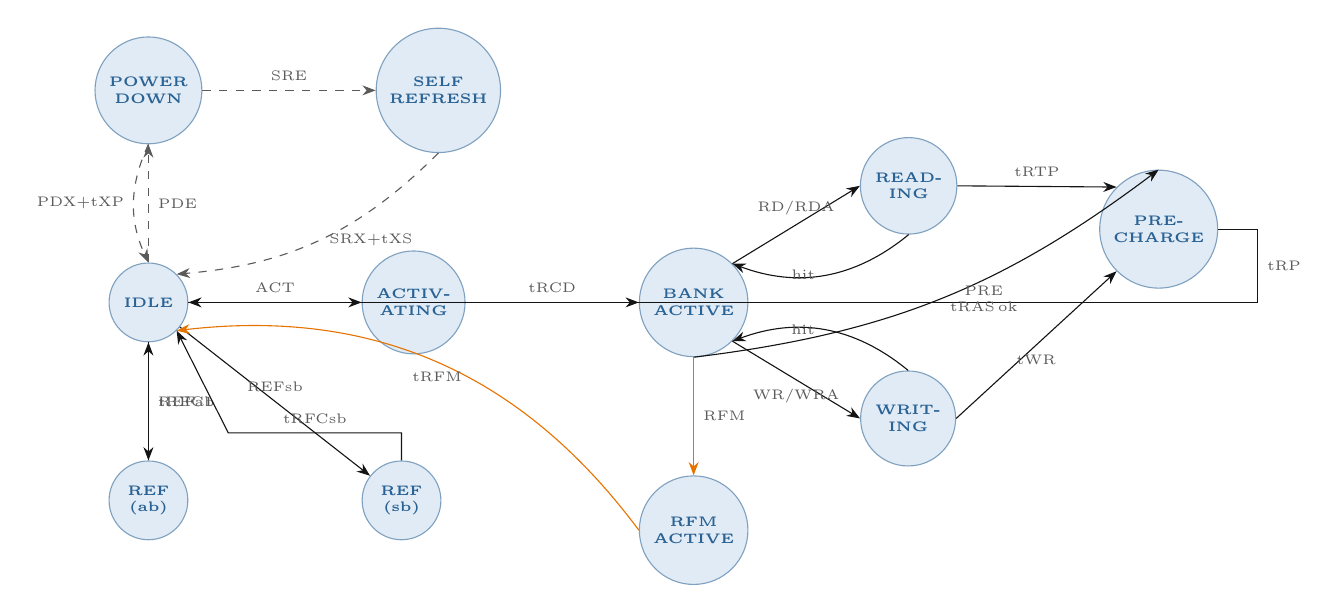
\begin{tikzpicture}[node distance=0.9cm and 2.0cm]

  %% core states — column layout
  \node[st] (idle) {IDLE};
  \node[st,right=2.2cm of idle]   (act)  {ACTIV-\\ATING};
  \node[st,right=2.2cm of act]    (ba)   {BANK\\ACTIVE};

  \node[st,above right=0.55cm and 1.8cm of ba] (rd)  {READ-\\ING};
  \node[st,below right=0.55cm and 1.8cm of ba] (wr)  {WRIT-\\ING};

  \node[st,right=1.8cm of rd,yshift=-0.55cm]  (pre) {PRE-\\CHARGE};

  %% refresh states below
  \node[st,below=1.5cm of idle]   (rab)  {REF\\(ab)};
  \node[st,right=2.2cm of rab]    (rsb)  {REF\\(sb)};

  %% power states above
  \node[st,above=1.5cm of idle]   (pd)   {POWER\\DOWN};
  \node[st,right=2.2cm of pd]     (sr)   {SELF\\REFRESH};

  %% RFM
  \node[st,below=1.5cm of ba]     (rfm)  {RFM\\ACTIVE};

  %% ── arrows ──────────────────────────────────────────────────────────────
  %% main path
  \draw[arr] (idle) -- node[above,lbl]{ACT} (act);
  \draw[arr] (act)  -- node[above,lbl]{tRCD} (ba);

  %% ba to RD/WR
  \draw[arr] (ba.north east) -- node[above,lbl]{RD/RDA} (rd.west);
  \draw[arr] (ba.south east) -- node[below,lbl]{WR/WRA} (wr.west);

  %% RD/WR to precharge
  \draw[arr] (rd.east) -- node[above,lbl]{tRTP} (pre.north west);
  \draw[arr] (wr.east) -- node[below,lbl]{tWR}  (pre.south west);

  %% row hits stay in BA
  \draw[arr,bend left=30] (rd.south) to node[left,lbl]{hit} (ba.north east);
  \draw[arr,bend right=30] (wr.north) to node[left,lbl]{hit} (ba.south east);

  %% PRE back to IDLE (route right-then-south-then-west)
  \draw[arr] (pre.east) -- ++(0.5,0) |- node[right,lbl,near start]{tRP} (idle.east);

  %% explicit PRE from BA
  \draw[arr,bend right=15] (ba.south) to node[right,lbl]{PRE\\tRAS\,ok} (pre.north);

  %% refresh
  \draw[arr] (idle.south) -- node[right,lbl]{REFab} (rab.north);
  \draw[arr] (rab.north)  -- node[right,lbl]{tRFC1} (idle.south);
  \draw[arr] (idle) -- node[above,lbl]{REFsb} (rsb);
  \draw[arr] (rsb.north) -- ++(0,0.35) -- node[above,lbl]{tRFCsb} ++(-2.2,0) -- (idle.south east);

  %% power down / SR
  \draw[darr] (idle.north) -- node[right,lbl]{PDE} (pd.south);
  \draw[darr] (pd.south) to[bend right=25] node[left,lbl]{PDX+tXP} (idle.north);
  \draw[darr] (pd.east) -- node[above,lbl]{SRE} (sr.west);
  \draw[darr] (sr.south) to[bend left=20] node[right,lbl]{SRX+tXS} (idle.north east);

  %% RFM
  \draw[aarr] (ba.south) -- node[right,lbl]{RFM} (rfm.north);
  \draw[aarr] (rfm.west) to[bend right=30] node[below,lbl]{tRFM} (idle.south east);

\end{tikzpicture}
\caption{Bank State Machine (single bank, 16 instances). Dashed arrows: CKE-controlled
         power transitions. Orange arrows: DDR5 RFM path.}
\end{figure}

\subsection{State Descriptions}

\begin{center}
\begin{tabularx}{\linewidth}{@{} l l X @{}}
\toprule
\Th{State} & \Th{Legal Inputs} & \Th{Timer / Exit} \\
\midrule
\RA IDLE              & ACT, REFab, REFsb, PDE, SRE, RFM & No timer. Exits on received command. \\
\RB ACTIVATING        & (internal)                        & tRCD countdown $\to$ BANK\_ACTIVE. \\
\RA BANK\_ACTIVE      & RD, RDA, WR, WRA, PRE, PREA       & tRAS loaded. PRE only after tRAS satisfied. Open row registered. \\
\RB READING           & BST                               & CL$+$BL/2. If RDA: hidden PRE starts at tRTP. \\
\RA WRITING           & BST                               & CWL$+$BL/2. If WRA: hidden PRE at CWL$+$BL/2. \\
\RB PRECHARGING       & ---                               & tRP counter $\to$ IDLE. \\
\RA REF (REFab)       & ---                               & tRFC1. All 16 banks locked simultaneously. \\
\RB REF (REFsb)       & ---                               & tRFCsb. Only target bank locked; others accessible. \\
\RA POWER DOWN        & PDX                               & Precharge PD (from IDLE) or Active PD (from ACTIVE). Exits after tXP. \\
\RB SELF REFRESH      & SRX                               & tCKSRE after CKE falls. SRX: tCKSRX, then tXS. \\
\RA RFM ACTIVE        & ---                               & tRFM (= tRFC1). Issued by RFM FSM when RAA $\leq$ RAAIMT. \\
\bottomrule
\end{tabularx}
\end{center}

\subsection{Per-Bank Timer Summary}

\begin{center}
\begin{tabularx}{0.92\linewidth}{@{} l l X @{}}
\toprule
\Th{Timer} & \Th{Loaded On} & \Th{Guards} \\
\midrule
\RA tRCD    & ACT issued   & First RD/WR on same bank \\
\RB tRAS    & ACT issued   & PRE/PREA on same bank (minimum open) \\
\RA tRC     & ACT issued   & Next ACT on same bank \\
\RB tRP     & PRE issued   & Next ACT on same bank \\
\RA tWR     & WR burst end & PRE on same bank \\
\RB tRTP    & RD issued    & PRE on same bank \\
\RA tRFC1   & REFab issued & Any command on any bank \\
\RB tRFCsb  & REFsb issued & Commands to refreshed bank only \\
\RA tXS     & SRX asserted & First ACT after self-refresh exit \\
\RB tXP     & PDX asserted & First command after power-down exit \\
\RA tMRD    & MRW issued   & Next MRW \\
\bottomrule
\end{tabularx}
\end{center}

%%%%%%%%%%%%%%%%%%%%%%%%%%%%%%%%%%%%%%%%%%%%%%%%%%%%%%%%%%%%%%%%%%%%%%%%%%%%
\section{Timing Control}
%%%%%%%%%%%%%%%%%%%%%%%%%%%%%%%%%%%%%%%%%%%%%%%%%%%%%%%%%%%%%%%%%%%%%%%%%%%%

Not a state machine. Combinational and registered timer array producing
\texttt{cmd\_ok[15:0][CMD\_TYPES]} every MC clock cycle. The Scheduler may only
issue a command when the corresponding \texttt{cmd\_ok} bit is asserted.

\subsection{Cross-Bank Constraint Checkers}

\begin{center}
\begin{tabularx}{\linewidth}{@{} l l X @{}}
\toprule
\Th{Constraint} & \Th{Scope} & \Th{Implementation} \\
\midrule
\RA tRRD\_L & Same BG, any bank & Timestamp of last ACT in BG. Block until $T_{now}-T_{last\_ACT\_BG}\geq t_{RRD\_L}$. \\
\RB tRRD\_S & Diff BG, any bank & Timestamp of last ACT globally. Block until $\Delta T\geq t_{RRD\_S}$. \\
\RA tFAW    & All banks, same rank & 4-entry ring buffer of ACT timestamps. Block if oldest is within tFAW. \\
\RB tCCD\_L & Same BG CAS & Last CAS in BG. Use tCCD\_L\_WR for WR; tCCD\_L\_WR2 for non-RMW WR. \\
\RA tCCD\_S & Diff BG CAS & Last CAS globally. $\Delta T\geq t_{CCD\_S}=\text{BL}/2$. \\
\RB tWTR\_L & Same BG, WR$\to$RD & Last WR data end in BG. Block RD until $\Delta T\geq WL+BL/2+t_{WTR\_L}$. \\
\RA tWTR\_S & Diff BG, WR$\to$RD & Same using $t_{WTR\_S}$. \\
\RB tRTW    & Any, RD$\to$WR     & Last RD cmd. Block WR until $\Delta T\geq RL+BL/2-WL+2+t_{WPRE}$. \\
\bottomrule
\end{tabularx}
\end{center}

%%%%%%%%%%%%%%%%%%%%%%%%%%%%%%%%%%%%%%%%%%%%%%%%%%%%%%%%%%%%%%%%%%%%%%%%%%%%
\section{DDR Command Scheduler}
%%%%%%%%%%%%%%%%%%%%%%%%%%%%%%%%%%%%%%%%%%%%%%%%%%%%%%%%%%%%%%%%%%%%%%%%%%%%

Arbitration heart of the MC Core. Consumes \texttt{cmd\_ok} from Timing Control,
bank states from BSMs, and pending transactions from RD/WR Cmd Pools.
Issues one DFI command per clock cycle.

\subsection{Scheduler FSM}

\begin{figure}[h]
\centering
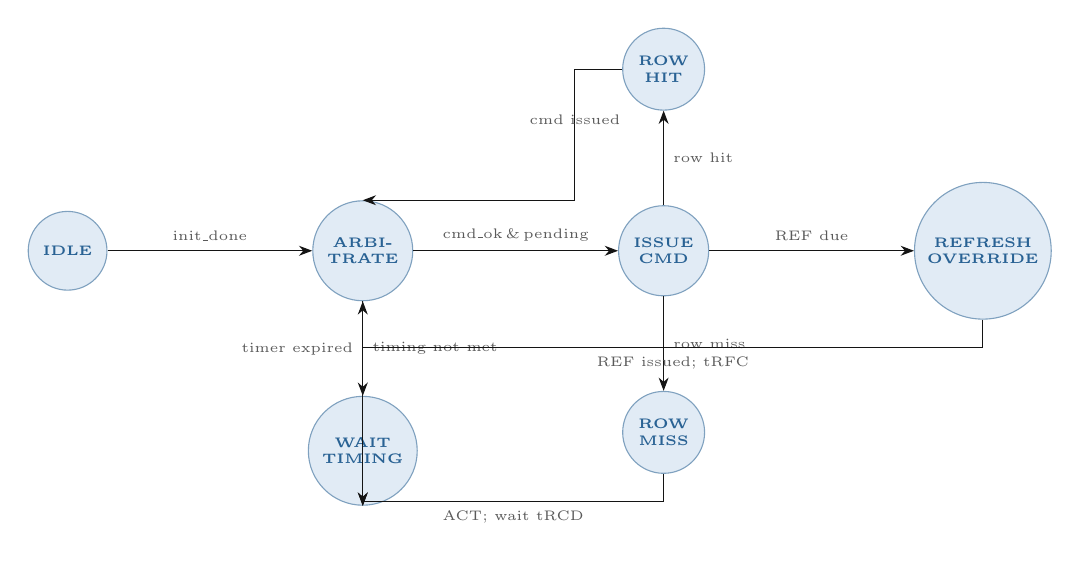
\begin{tikzpicture}[node distance=0.9cm and 2.4cm]
  \node[st] (idle)  {IDLE};
  \node[st,right=2.6cm of idle]  (arb)   {ARBI-\\TRATE};
  \node[st,right=2.6cm of arb]   (issue) {ISSUE\\CMD};
  \node[st,below=1.2cm of arb]   (wait)  {WAIT\\TIMING};
  \node[st,above=1.2cm of issue] (hit)   {ROW\\HIT};
  \node[st,below=1.2cm of issue] (miss)  {ROW\\MISS};
  \node[st,right=2.6cm of issue] (ref)   {REFRESH\\OVERRIDE};

  \draw[arr] (idle)--(arb)       node[above,lbl,midway]{init\_done};
  \draw[arr] (arb)--(issue)      node[above,lbl,midway]{cmd\_ok\,\&\,pending};
  \draw[arr] (arb)--(wait)       node[right,lbl,midway]{timing not met};
  \draw[arr] (wait)--(arb)       node[left,lbl,midway]{timer expired};
  \draw[arr] (issue.north)--(hit.south)  node[right,lbl,midway]{row hit};
  \draw[arr] (issue.south)--(miss.north) node[right,lbl,midway]{row miss};
  \draw[arr] (hit.west)  -- ++(-0.6,0) |- node[above,lbl,near start]{cmd issued} (arb.north);
  \draw[arr] (miss.south) -- ++(0,-0.35) -| node[below,lbl,near start]{ACT; wait tRCD} (wait.south);
  \draw[arr] (issue.east)--(ref.west)    node[above,lbl,midway]{REF due};
  \draw[arr] (ref.south)  -- ++(0,-0.35) -| node[below,lbl,near start]{REF issued; tRFC} (wait.south);
\end{tikzpicture}
\caption{DDR Command Scheduler FSM. One command per MC clock cycle.}
\end{figure}

\subsection{Command Priority Order}

\begin{enumerate}
  \item Refresh Override --- REF budget about to expire (highest priority)
  \item RFM --- RAA\,$\leq$\,RAAIMT (safety critical)
  \item ZQcal --- periodic; low urgency until overdue
  \item Write drain --- write buffer nearly full
  \item Row-hit reads --- open page, same row
  \item Row-hit writes
  \item Row-miss reads --- ACT $\to$ wait tRCD $\to$ RD
  \item Row-miss writes
  \item PRE --- close idle banks in closed-page mode
\end{enumerate}

\subsection{Page Policy}

\begin{center}
\begin{tabularx}{\linewidth}{@{} l l l X @{}}
\toprule
\Th{Policy} & \Th{Row Hit} & \Th{Row Miss} & \Th{Best For} \\
\midrule
\RA Open Page  & CAS only     & PRE\,$\xrightarrow{tRP}$\,ACT\,$\xrightarrow{tRCD}$\,CAS & Sequential / high locality \\
\RB Closed Page& ACT$+$CAS    & ACT\,$\xrightarrow{tRCD}$\,CAS                           & Random / streaming \\
\RA Adaptive   & Hit-rate decides & Sliding window $N=256$ & Mixed; autotunes per bank \\
\bottomrule
\end{tabularx}
\end{center}

\subsection{Arbitration Logic}

\begin{center}
\begin{tabularx}{\linewidth}{@{} c l l X @{}}
\toprule
\Th{Level} & \Th{Winner} & \Th{Condition} & \Th{Effect} \\
\midrule
\RA 0 & REF urgent   & Credits $\geq 8$ or $\Delta t_{since REF}>t_{REFI\_max}$ & Hard stall; all RD/WR suppressed \\
\RB 1 & REF nominal  & tREFI countdown reaches zero    & REF injected; RD/WR deferred \\
\RA 2 & ZQ cal       & tZQCS interval expires          & ZQCS after current REF \\
\RB 3 & Read         & RD pool non-empty \& RD mode    & BG-aware scheduling \\
\RA 4 & Write        & WR pool non-empty \& WR mode    & Watermark-controlled batching \\
\RB 5 & Scrubber/MRR & Background idle slot            & Pre-emptible \\
\bottomrule
\end{tabularx}
\end{center}

\textbf{Anti-starvation:} age counter per entry. At AGE\_THR1 (64\,cy): intra-class HOL bypass.
At AGE\_THR2 (256\,cy): WR may overtake RD priority. Resets to 0 on dispatch.

\textbf{RD/WR mode switching:} switch to WR mode when WR depth\,$\geq$\,WR\_HIGH\_WM (32) or
RD empty. Switch back when WR depth\,$\leq$\,WR\_LOW\_WM (8) or WR empty or urgent RD.
Hysteresis gap of 24 entries prevents mode thrashing.

\subsection{Command Selector --- Legal Check Matrix}

All gates checked before dispatch. Any false bit $\Rightarrow$ NOP inserted that cycle.

\begin{center}
\begin{tabularx}{\linewidth}{@{} l l X @{}}
\toprule
\Th{Gate} & \Th{Timer Source} & \Th{Constraint} \\
\midrule
\RA \texttt{bank\_avail[b]}   & BSM state         & Bank not in ACTIVATING or PRECHARGING \\
\RB \texttt{gate\_rcd[b]}     & ACT issue         & $t_{RCD}$: ACT to first CAS on same bank \\
\RA \texttt{gate\_rp[b]}      & PRE issue         & $t_{RP}$: PRE to ACT on same bank \\
\RB \texttt{gate\_ras[b]}     & ACT issue         & $t_{RAS}$: ACT to PRE minimum \\
\RA \texttt{gate\_ccd\_l}     & Same BG CAS       & $t_{CCD\_L}$ or $t_{CCD\_L\_WR}$ or $t_{CCD\_L\_WR2}$ \\
\RB \texttt{gate\_ccd\_s}     & Diff BG CAS       & $t_{CCD\_S}=\text{BL}/2$ \\
\RA \texttt{gate\_rrd\_l}     & Same BG ACT       & $t_{RRD\_L}$ \\
\RB \texttt{gate\_rrd\_s}     & Diff BG ACT       & $t_{RRD\_S}$ \\
\RA \texttt{gate\_faw}        & Sliding window    & $\leq$4 ACTs within $t_{FAW}$ \\
\RB \texttt{gate\_wtr\_l}     & WR data end, same BG & $t_{WTR\_L}$: WR to RD \\
\RA \texttt{gate\_wtr\_s}     & WR data end, diff BG & $t_{WTR\_S}$: WR to RD \\
\RB \texttt{gate\_rtw}        & RD cmd            & $t_{RTW}=RL+BL/2+2-WL$ \\
\RA \texttt{gate\_rfc[r]}     & REF issue, per rank & $t_{RFC1}$: all commands blocked \\
\RB \texttt{gate\_rfcpb[r][b]}& REFsb, per bank   & $t_{RFCsb}$: same bank blocked \\
\RA \texttt{gate\_zqcs}       & ZQCS issue        & All commands blocked during ZQ \\
\RB \texttt{gate\_mrd}        & MRW issue         & $t_{MRD}$: MRW-to-MRW \\
\bottomrule
\end{tabularx}
\end{center}

%%%%%%%%%%%%%%%%%%%%%%%%%%%%%%%%%%%%%%%%%%%%%%%%%%%%%%%%%%%%%%%%%%%%%%%%%%%%
\section{Maintenance Engine}
%%%%%%%%%%%%%%%%%%%%%%%%%%%%%%%%%%%%%%%%%%%%%%%%%%%%%%%%%%%%%%%%%%%%%%%%%%%%

Four independent sub-FSMs handle all autonomous background operations. Each posts requests
to the Cmd Scheduler via a priority request bus.

\subsection{Refresh Scheduler FSM}

\begin{figure}[h]
\centering
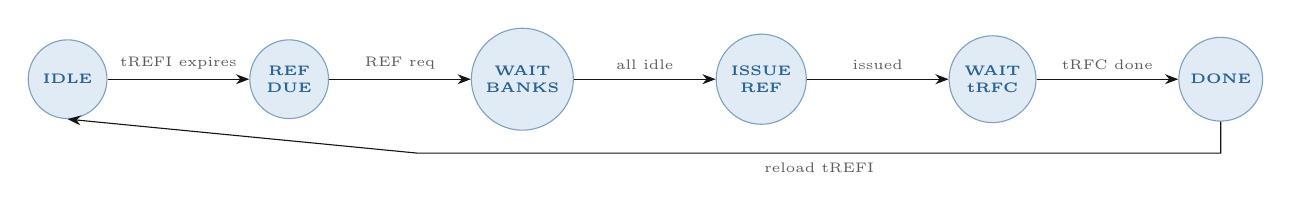
\begin{tikzpicture}[node distance=0.55cm and 1.6cm]
  \node[st] (idle)  {IDLE};
  \node[st,right=1.8cm of idle]   (due)   {REF\\DUE};
  \node[st,right=1.8cm of due]    (wait)  {WAIT\\BANKS};
  \node[st,right=1.8cm of wait]   (issue) {ISSUE\\REF};
  \node[st,right=1.8cm of issue]  (wrfc)  {WAIT\\tRFC};
  \node[st,right=1.8cm of wrfc]   (done)  {DONE};

  \draw[arr] (idle)--(due)   node[above,lbl,midway]{tREFI expires};
  \draw[arr] (due)--(wait)   node[above,lbl,midway]{REF req};
  \draw[arr] (wait)--(issue) node[above,lbl,midway]{all idle};
  \draw[arr] (issue)--(wrfc) node[above,lbl,midway]{issued};
  \draw[arr] (wrfc)--(done)  node[above,lbl,midway]{tRFC done};
  \draw[arr] (done.south) -- ++(0,-0.4) -- node[below,lbl]{reload tREFI} ++(-10.2,0) -- (idle.south);
\end{tikzpicture}
\caption{Refresh Scheduler FSM. REFsb path substitutes WAIT\_TARGET\_BANK for WAIT\_BANKS
         and uses tRFCsb. FGR mode replaces tRFC1 with tRFC2/tRFC4.}
\end{figure}

\begin{itemize}
  \item \textbf{Leaky-bucket:} +1 each tREFI, $-1$ on REF issued. Counter $\geq$9: \texttt{ref\_urgent} asserted.
  \item \textbf{REFsb cycling:} BA[1:0] cycles $00\to01\to10\to11$. 8 REFsb $\approx$ 1 REFab credit.
  \item \textbf{FGR:} REF\_MODE[1]=1 $\Rightarrow$ tRFC2; REF\_MODE=11 $\Rightarrow$ tRFC4. Budget threshold halved/quartered.
  \item \textbf{Temperature derating:} MR4 TUF=1 $\Rightarrow$ tREFI halved. MC polls MR4 via background MRR.
\end{itemize}

\subsection{ZQcal FSM}

States: IDLE $\to$ WAIT\_IDLE $\to$ ISSUE\_ZQCAL\_START $\to$ WAIT\_tZQCAL $\to$
ISSUE\_ZQCAL\_LATCH $\to$ WAIT\_tZQLAT $\to$ DONE $\to$ IDLE.

Triggered by periodic tZQCS timer or host \texttt{ZQCAL\_TRIG} bit. All banks must be idle.
During ZQCAL, all commands blocked via \texttt{gate\_zqcs}.

\begin{center}
\begin{tabularx}{0.75\linewidth}{@{} l r l @{}}
\toprule
\Th{Parameter} & \Th{Value} & \Th{Description} \\
\midrule
\RA $t_{ZQCAL}$ & 1\,$\mu$s   & ZQCAL Start to Latch \\
\RB $t_{ZQLAT}$ & 30\,nCK     & Latch to next command \\
\RA $t_{ZQCS\_INT}$ & $\sim$128\,ms & Periodic interval (CSR-configurable) \\
\bottomrule
\end{tabularx}
\end{center}

\subsection{RFM FSM}

States: IDLE $\to$ MONITOR\_RAA $\to$ RFM\_REQUEST $\to$ WAIT\_ISSUE $\to$
WAIT\_tRFM $\to$ UPDATE\_RAA $\to$ MONITOR\_RAA.

\begin{itemize}
  \item RAA[b] $+=1$ on every ACT to bank $b$; RAA[b] $-=$ RAADec on every REF to bank $b$.
  \item RAA[b] $\leq$ RAAIMT: assert RFM request (priority above ZQcal, below refresh override).
  \item tRFM $=$ tRFC1. Bank enters RFM\_ACTIVE. After tRFM: RAA[b] reset to RAAIMT.
\end{itemize}

\subsection{Power Management FSM}

States: NORMAL $\to$ PD\_ENTRY\_CHECK $\to$ \{PRECHARGE\_PD\,|\,ACTIVE\_PD\} $\to$
PDX\_WAIT\_tXP $\to$ NORMAL.

SR branch: NORMAL $\to$ SR\_ENTRY $\to$ WAIT\_tCKSRE $\to$ SELF\_REFRESHING $\to$
SR\_EXIT $\to$ WAIT\_tCKSRX $\to$ WAIT\_tXS $\to$ WAIT\_tDLLK $\to$ NORMAL.

MPSM: MR2 OP[1:0]=01. Deeper than SR. Exit via DES then MRW to clear.

%%%%%%%%%%%%%%%%%%%%%%%%%%%%%%%%%%%%%%%%%%%%%%%%%%%%%%%%%%%%%%%%%%%%%%%%%%%%
\section{Write Data Path}
%%%%%%%%%%%%%%%%%%%%%%%%%%%%%%%%%%%%%%%%%%%%%%%%%%%%%%%%%%%%%%%%%%%%%%%%%%%%

\begin{center}
\begin{tabularx}{\linewidth}{@{} l X @{}}
\toprule
\Th{Sub-Block} & \Th{Description} \\
\midrule
\RA Write Data Buffer & BL16-aligned FIFO. Stores write data from CIF Write Cmd Pool via CDC.
  Dequeued when Scheduler confirms a write slot. \\
\RB DM/ECC Generator & Per-byte Data Mask. Inline Write CRC using $G(x)=x^4+x+1$ over DQ+DM
  bits per BL16 burst. Enabled via MR8 OP[6]=1. \\
\RA WL Align & Programmable pipeline delay $=$ CWL to align DQS preamble to
  \texttt{dfi\_wrdata\_en}. Offset from PHY\_WRLAT. \\
\RB DFI Write Timing & Drives \texttt{dfi\_wrdata[127:0]}, \texttt{dfi\_wrdata\_mask[15:0]},
  \texttt{dfi\_wrdata\_cs\_n}, \texttt{dfi\_parity\_in}. Preamble per MR8 (2\,tCK).
  ODT: $t_{ODTon}=WL-2$, $t_{ODToff}=WL+BL/2$. \\
\RA Write CRC FSM & NORMAL $\to$ CRC\_ERROR $\to$ RETRY\_WRITE $\to$ AUTO\_DISABLE.
  Monitors \texttt{dfi\_alert\_n}. Retries up to $n$ times; auto-disables CRC via MRW to MR8. \\
\bottomrule
\end{tabularx}
\end{center}

%%%%%%%%%%%%%%%%%%%%%%%%%%%%%%%%%%%%%%%%%%%%%%%%%%%%%%%%%%%%%%%%%%%%%%%%%%%%
\section{Read Data Path}
%%%%%%%%%%%%%%%%%%%%%%%%%%%%%%%%%%%%%%%%%%%%%%%%%%%%%%%%%%%%%%%%%%%%%%%%%%%%

\begin{center}
\begin{tabularx}{\linewidth}{@{} l X @{}}
\toprule
\Th{Sub-Block} & \Th{Description} \\
\midrule
\RA Read Latency Counter & Per-outstanding-read counter. Tracks CL + read preamble from RD
  command to expected DFI data arrival. Issues \texttt{dfi\_rddata\_en} PHY\_RDLAT cycles early. \\
\RB Read Data FIFO & Captures \texttt{dfi\_rddata[127:0]} on \texttt{dfi\_rddata\_valid}.
  Re-aligns per-burst data. Feeds CIF Reorder Buffer with AXI transaction tag. \\
\RA ECC/CRC Checker & Verifies Read CRC when MR8 OP[7]=1. On error: flags to CIF error register;
  optionally triggers read retry. Adds RL latency per JESD79-5 Table\,365. \\
\RB ECS FSM & IDLE $\to$ ECS\_ACTIVE $\to$ WAIT\_tECS $\to$ IDLE. Triggered by MR14 or host
  MPC. DRAM scrubs on-die ECC during tECS ($\leq t_{RFC1}$). Logs in MR16--MR20. \\
\bottomrule
\end{tabularx}
\end{center}

%%%%%%%%%%%%%%%%%%%%%%%%%%%%%%%%%%%%%%%%%%%%%%%%%%%%%%%%%%%%%%%%%%%%%%%%%%%%
\section{DFI 5.2 Interface}
%%%%%%%%%%%%%%%%%%%%%%%%%%%%%%%%%%%%%%%%%%%%%%%%%%%%%%%%%%%%%%%%%%%%%%%%%%%%

\texttt{dfi\_wrdata\_en} asserted PHY\_WRLAT cycles before write data.
\texttt{dfi\_rddata\_valid} arrives PHY\_RDLAT cycles after the RD command.
Both offsets set during DFI training. FREQ\_RATIO determines nCK per DFI clock.

\begin{center}
\begin{tabularx}{\linewidth}{@{} l l X @{}}
\toprule
\Th{Signal} & \Th{Dir} & \Th{Description} \\
\midrule
\RA \texttt{dfi\_address[13:0]}    & MC$\to$PHY & CA bus. 2-cycle encoding for DDR5 ACT. \\
\RB \texttt{dfi\_cs\_n[1:0]}       & MC$\to$PHY & Chip select per rank. \\
\RA \texttt{dfi\_cke[1:0]}         & MC$\to$PHY & Clock Enable per rank. \\
\RB \texttt{dfi\_odt[1:0]}         & MC$\to$PHY & On-Die Termination control per rank. \\
\RA \texttt{dfi\_reset\_n}         & MC$\to$PHY & DRAM RESET\_n. Driven by Init FSM. \\
\RB \texttt{dfi\_act\_n}           & MC$\to$PHY & Activate indicator (DDR5). \\
\RA \texttt{dfi\_bank[1:0]}        & MC$\to$PHY & Bank address. \\
\RB \texttt{dfi\_bg[2:0]}          & MC$\to$PHY & Bank group. BG[2:0] x4/x8; BG[1:0] x16. \\
\RA \texttt{dfi\_wrdata[127:0]}    & MC$\to$PHY & Write data (BL16\,$\times$\,DQ8). \\
\RB \texttt{dfi\_wrdata\_mask[15:0]}& MC$\to$PHY & Write data mask per byte lane. \\
\RA \texttt{dfi\_wrdata\_en}       & MC$\to$PHY & Asserted PHY\_WRLAT cycles early. \\
\RB \texttt{dfi\_wrdata\_cs\_n}    & MC$\to$PHY & Per-DRAM write chip select (DDR5 PDA). \\
\RA \texttt{dfi\_parity\_in}       & MC$\to$PHY & CA parity bit (DDR5). \\
\RB \texttt{dfi\_rddata[127:0]}    & PHY$\to$MC & Captured read data. \\
\RA \texttt{dfi\_rddata\_valid}    & PHY$\to$MC & Read data valid. \\
\RB \texttt{dfi\_rddata\_dnv}      & PHY$\to$MC & Data-not-valid error. \\
\RA \texttt{dfi\_alert\_n}         & PHY$\to$MC & DRAM alert: Write CRC or CA parity error. \\
\RB \texttt{dfi\_ctrlupd\_req/ack} & both & Controller-initiated PHY update handshake. \\
\RA \texttt{dfi\_phyupd\_req/ack}  & both & PHY-initiated update/pause handshake. \\
\RB \texttt{dfi\_init\_start/complete}& both & Init FSM PHY initialization handshake. \\
\RA \texttt{dfi\_freq\_ratio[1:0]} & MC$\to$PHY & 00=1:1, 01=1:2, 10=1:4. \\
\bottomrule
\end{tabularx}
\end{center}

%%%%%%%%%%%%%%%%%%%%%%%%%%%%%%%%%%%%%%%%%%%%%%%%%%%%%%%%%%%%%%%%%%%%%%%%%%%%
\section{FSM Inventory}
%%%%%%%%%%%%%%%%%%%%%%%%%%%%%%%%%%%%%%%%%%%%%%%%%%%%%%%%%%%%%%%%%%%%%%%%%%%%

\begin{center}
\begin{tabularx}{0.9\linewidth}{@{} l r r X @{}}
\toprule
\Th{FSM} & \Th{States} & \Th{Inst.} & \Th{Notes} \\
\midrule
\RA Init FSM              & 16 & 1  & RESET\_n through training complete \\
\RB Bank State Machine    & 11 & 16 & One per bank; 176 total state bits \\
\RA Arbitration Logic     & 6  & 1  & RD/WR mode + priority selection \\
\RB Command Selector      & 4  & 1  & Page policy + legal check + seq gen \\
\RA Refresh Scheduler     & 7  & 1  & REFab + REFsb + FGR + urgent override \\
\RB ZQcal FSM             & 7  & 1  & MPC ZQCAL Start/Latch flow \\
\RA RFM FSM               & 6  & 1  & Per-bank RAA monitoring + RFM injection \\
\RB Power Management FSM  & 10 & 1  & PD (Pre/Act), SR, MPSM \\
\RA Write CRC Error FSM   & 4  & 1  & \texttt{dfi\_alert\_n} monitoring; retry + auto-disable \\
\RB ECS FSM               & 4  & 1  & DDR5 inline ECC scrub window \\
\midrule
\RA \textbf{Total}        & \textbf{$\approx$75} & \textbf{23} & \\
\bottomrule
\end{tabularx}
\end{center}

%%%%%%%%%%%%%%%%%%%%%%%%%%%%%%%%%%%%%%%%%%%%%%%%%%%%%%%%%%%%%%%%%%%%%%%%%%%%
\section{Timing Reference}
%%%%%%%%%%%%%%%%%%%%%%%%%%%%%%%%%%%%%%%%%%%%%%%%%%%%%%%%%%%%%%%%%%%%%%%%%%%%

Values at 200\,MHz (tCK\,=\,5\,ns, CL\,=\,3, CWL\,=\,1, BL/2\,=\,8) and 100\,MHz.
Production values set via Config Regs from actual speed bin.

\begin{center}
\begin{tabularx}{\linewidth}{@{} l l r r @{}}
\toprule
\Th{Command Sequence} & \Th{Formula} & \Th{@200\,MHz} & \Th{@100\,MHz} \\
\midrule
\RA ACT $\to$ RD/WR (same bank) & tRCD & 4 & 4 \\
\RB ACT $\to$ PRE (same bank, min) & tRAS & 7 & 4 \\
\RA PRE $\to$ ACT (same bank) & tRP & 4 & 4 \\
\RB ACT $\to$ ACT (same bank) & tRC\,=\,tRAS+tRP & 11 & 8 \\
\RA ACT $\to$ ACT (same BG) & tRRD\_L & 4 & 4 \\
\RB ACT $\to$ ACT (diff BG) & tRRD\_S & 2 & 2 \\
\RA RD $\to$ RD (same BG) & tCCD\_L & 8 & 8 \\
\RB WR $\to$ WR (same BG) & tCCD\_L\_WR & 32 & 32 \\
\RA WR $\to$ WR same BG (not RMW) & tCCD\_L\_WR2 & 16 & 16 \\
\RB RD/WR (diff BG) & tCCD\_S\,=\,BL/2 & 8 & 8 \\
\RA RD $\to$ WR (any) & RL+BL/2$-$WL+2+tWPRE & 14 & 14 \\
\RB WR $\to$ RD (same BG) & WL+BL/2+tWTR\_L & 13 & 13 \\
\RA WR $\to$ RD (diff BG) & WL+BL/2+tWTR\_S & 11 & 11 \\
\RB REFab $\to$ any & tRFC1 & 39 & 20 \\
\RA SRX $\to$ ACT & tXS\,=\,tRFC1+10\,ns & 41 & 21 \\
\RB ZQCAL Start $\to$ Latch & tZQCAL\,=\,1\,$\mu$s & 200 & 100 \\
\RA 4 ACT window & tFAW & 16 & 16 \\
\bottomrule
\end{tabularx}
\end{center}

%%%%%%%%%%%%%%%%%%%%%%%%%%%%%%%%%%%%%%%%%%%%%%%%%%%%%%%%%%%%%%%%%%%%%%%%%%%%
\section{DDR5 vs DDR4 --- Design Deltas}
%%%%%%%%%%%%%%%%%%%%%%%%%%%%%%%%%%%%%%%%%%%%%%%%%%%%%%%%%%%%%%%%%%%%%%%%%%%%

\begin{center}
\begin{tabularx}{\linewidth}{@{} l l X @{}}
\toprule
\Th{Feature} & \Th{DDR4} & \Th{DDR5 MC Core Impact} \\
\midrule
\RA BL              & BL8 (BL/2=4)      & BL16 (BL/2=8). All RTW, WTR, WR-to-PRE formulae scale by 2. \\
\RB ACT encoding    & 1-cycle CA        & 2-cycle CA. Scheduler drives CA on two consecutive rising edges. \\
\RA REFsb           & Not supported     & Refresh Scheduler adds REFsb path; per-bank tRFCsb in BSM. \\
\RB RFM             & Not supported     & Full RFM FSM; per-bank RAA counters; RAAIMT/RAAMMT in Config Regs. \\
\RA ZQ mechanism    & ZQCL/ZQCS cmds   & MPC ZQCAL Start+Latch. Init FSM restructured; ZQcal FSM uses MPC. \\
\RB tRFC1 (8\,Gb)   & 350\,ns           & 195\,ns. Shorter penalty; more scheduling headroom. \\
\RA tREFI           & 7.8\,$\mu$s       & 3.9\,$\mu$s. Double refresh rate; budget counter threshold halved. \\
\RB CWL             & Separate lookup   & CWL = CL$-$2 fixed. Simplifies Config Reg and RTW formula. \\
\RA tMOD            & 24\,nCK after MRS & Replaced by tMRD only (16\,nCK). No separate tMOD path. \\
\RB tCCD\_L\_WR     & Not defined       & max(32\,nCK,\,20\,ns). New gate in Command Selector. \\
\RA Write CRC       & Optional (MR5)    & Mandatory support. \texttt{dfi\_alert\_n} monitoring; Write CRC FSM. \\
\RB ECS             & Not supported     & ECS FSM in Read Data Path; hooks into tRFC window. \\
\RA MR addressing   & 3 MRs             & 256 MRs via MRW/MRR. Init FSM MRW burst extended. \\
\bottomrule
\end{tabularx}
\end{center}

\vspace{10pt}
\noindent\color{acc1!40}\rule{\linewidth}{0.5pt}\\[2pt]
{\small\color{notetext}
MC Core Design Specification\,---\,Memory Controller Capstone Project.
JEDEC JESD79-5 (DDR5) / DFI\,5.2 / AXI4.
Timing values device-specific; validate against datasheet per speed bin.}

\end{document}
